\section{Evaluation}\label{sec:eval}


In this section, we evaluate \sysname on both benchmarks and real-world IoT devices in terms of its correctness, performance and effectiveness.

%First, we evaluate \sysname on 4 GNU core utilities programs from LAVA-M dataset to see if \sysname can indeed find bugs inside programs. 

%Then, we use the same 4 programs to evaluate its performance by running both \sysname instrumented binaries and AFL compiled binaries for each of the program with a fixed amount of time. To minimize the randomness AFL introduces, each program was evaluated several times. 


\subsection{Evaluation on Benchmarks}

As mentioned in previous sections, \sysname allows coverage-based fuzzers~(e.g. AFL) to run on Linux-based IoT devices by implementing binary level instrumentation. Although our approach does not involve any modification to fuzzing strategy of the original fuzzer, we leverage a well-known fuzzer benchmark: LAVA-M~\cite{dolan2016lava} to evaluate its correctness and performance. 

\subsubsection{Correctness}
To verify the correctness of our approach, we need to run \sysname on a dataset with ground-truth to see if it can correctly fuzz a program and find bugs. LAVA-M is a widely-used fuzzer benchmark that automatically injects a large number of bugs into four GNU core utilities programs: $uniq$, $base64$, $who$ and $md5sum$. We selected the $uniq$ program to compare AFL and \sysname. Since AFL cannot run on real device, we ran this experiment on Ubuntu 16.04 in the QEMU-ARM emulator, where each host is configured with 2 cores and 4GB memory. 

% However, existing research~\cite{chen2018angora} shows that AFL does not perform well on all these four programs in LAVA-M dataset and it can only find certain number of bugs within program uniq and almost none within others. Given that \sysname simply integrates AFL to generate input and does not optimize AFL’s fuzzing strategy, we certainly cannot expect it to find more bugs than AFL. 

We ran two experiments on $uniq$ program in parallel, one using AFL and the other using \sysname. To mitigate the impact of randomization during fuzzing, we repeated each experiment six times. In the experiment with AFL, we first compiled the $uniq$ program from the source code with afl-clang-fast and then ran it with AFL on a single core for 10 hours. AFL performs a LLVM level instrumentation during compilation. In comparison, our \sysname experiment performed binary level instrumentation on a pre-compiled version of $uniq$ program. We compiled it using the same source code and parameters of afl-clang-fast as in the AFL experiment. Similarly, the experiment lasted for 10 hours on a single core.

We used several metrics provided by AFL to measure the fuzzing process. First, the number of unique crashes indicates the identified bugs. Second, the branch coverage indicates the proportion of branches that were executed in the fuzzing process. Third, the number of total path reflects the number of unique execution paths triggered by fuzzer. Table~\ref{table:res_comp} shows that the \sysname and AFL experiments have similar results, which demonstrates the correctness of \sysname.

%We first compile the uniq program with afl-clang-fast, which comes with AFL, and then run AFL for about 10 hours on a single core. In order to eliminate the impact of AFL's random mutation, we repeat the experiment three times to get the following results. The first experiment triggered 6 unique crashes, and the third triggered 4. The detailed results are illustrated in Table~\ref{table:res_afl}.

%In comparison, we use clang to compile uniq with the same parameters as afl-clang-fast and then instrument the target binary with \sysname. We test instrumented program for a total of 6 times, giving each fuzz instance about 10 hours of running time on a single core. In 6 sets of tests~(See Table~\ref{table:res_ours}), we can find crashes every time, and up to 6 unique Crashes can be triggered. The results of the test, including bitmap coverage and total paths found, are basically the same as those of the AFL compiled program. This result proves the correctness of \sysname, which is quite the same as AFL with source code.

%In other work (Angora), AFL found 9 unique crashes in uniq when the single core was running for 5 hours. Although the result in our experiment is not as good as theirs but noticed that we are running under emulation, which is much slower than a real x86 environment.


\begin{table}
\scriptsize
\renewcommand\arraystretch{1.2}
\center
\begin{threeparttable}
\begin{tabular}
{
|C{0.05\textwidth}
|C{0.045\textwidth}
|C{0.045\textwidth}
|C{0.055\textwidth}
|C{0.03\textwidth}
|C{0.05\textwidth}
|
}
%\toprule
\hline
\rmfamily\textbf{Tool}&
\rmfamily\textbf{\# of Run}&
\rmfamily\textbf{\# of Unique Crash}&
\rmfamily\textbf{Branch Coverage}&
\rmfamily\textbf{\# of Total Path} &
\rmfamily\textbf{Execution Time~(H)}
\\
%\midrule
\hline
\multirow{6}*{AFL} &
1 & 6 & 29.82\% & 75 & 10 \\
\cline{2-6}
~& 2 & 0 & 29.82\% & 80 & 10 \\
\cline{2-6}
~&3 & 4 & 29.82\% & 77 & 10 \\
\cline{2-6}
~&4 & 0 & 29.82\% & 78 & 10 \\
\cline{2-6}
~&5 & 4 & 29.82\% & 83 & 10 \\
\cline{2-6}
~&6 & 4 & 29.82\% & 71 & 10 \\
\hline

\multirow{6}*{\sysname} &
1 & 6 & 29.64\% & 79 & 10 \\
\cline{2-6}
~ & 2 & 1 & 29.64\% & 76 & 10 \\
\cline{2-6}
~ &3 & 1 & 29.64\% & 74 & 10 \\
\cline{2-6}
~ &4 & 4 & 29.64\% & 82 & 10 \\
\cline{2-6}
~ &5 & 3 & 29.64\% & 76 & 10 \\
\cline{2-6}
~ &6 & 1 & 29.64\% & 78 & 10 \\
\hline
\end{tabular}

%\footnotesize
%\item[1] APIs of embedded ad are found in both in Java code~(299 APIs) and XML~(108 APIs) layout resource files in apps~(Listing~\ref{lst:bannerlayout1} and Listing~\ref{lst:bannerlayout2}).
%\end{tablenotes}
\end{threeparttable}
\caption{\label{table:res_comp}Fuzzing Test Result on $uniq$ in Lava-M Dataset with AFL and \sysname.}
\end{table}

% \begin{table}
% %\ttfamily
% \scriptsize
% \renewcommand\arraystretch{1.2}
% \center
% \begin{threeparttable}
% \begin{tabular}
% {
% |C{0.05\textwidth}
% |C{0.05\textwidth}
% |C{0.1\textwidth}
% |C{0.05\textwidth}
% |C{0.1\textwidth}
% |
% }
% %\toprule
% \hline
% \rmfamily\textbf{Number of Run}&
% \rmfamily\textbf{Unique Crashes}&
% \rmfamily\textbf{Bitmap Coverage}&
% \rmfamily\textbf{Total Paths} &
% \rmfamily\textbf{Execution Time~(H)}
% \\
% %\midrule
% \hline
% 1 & 6 & 0.44\% & 79 & 10 \\
% \hline
% 2 & 1 & 0.44\% & 76 & 10 \\
% \hline
% 3 & 1 & 0.44\% & 74 & 10 \\
% \hline
% 4 & 4 & 0.44\% & 82 & 10 \\
% \hline
% 5 & 3 & 0.44\% & 76 & 10 \\
% \hline
% 6 & 1 & 0.44\% & 78 & 10 \\
% \hline
% \end{tabular}
% %\footnotesize
% %\item[1] APIs of embedded ad are found in both in Java code~(299 APIs) and XML~(108 APIs) layout resource files in apps~(Listing~\ref{lst:bannerlayout1} and Listing~\ref{lst:bannerlayout2}).
% %\end{tablenotes}
% \end{threeparttable}
% \caption{\label{table:res_ours}Fuzzing Test Result on $uniq$ in Lava-M Dataset with \sysname.}
% \end{table}


\begin{figure}[htbp]
\centering

\begin{subfigure}[b]{0.48\textwidth}
       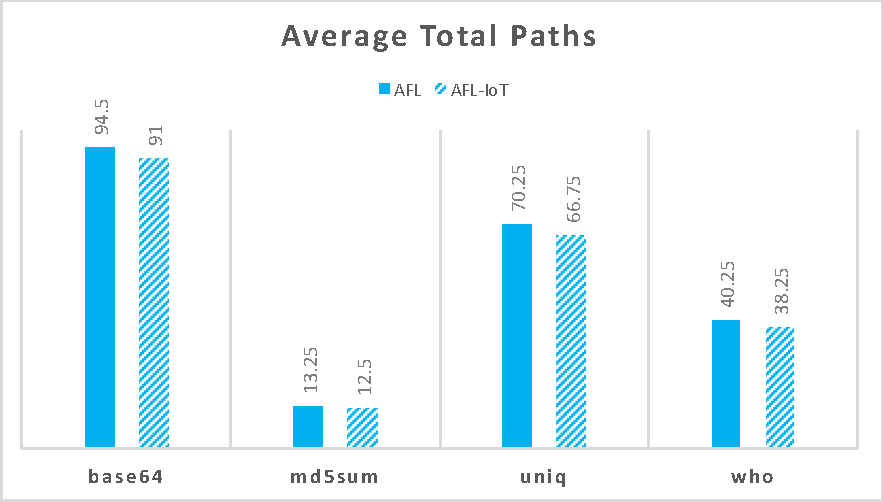
\includegraphics[width=\textwidth]{paths}
        \caption{Average Total Paths}
    \end{subfigure}%
\vspace{5pt}
%\begin{subfigure}[b]{0.48\textwidth}
%        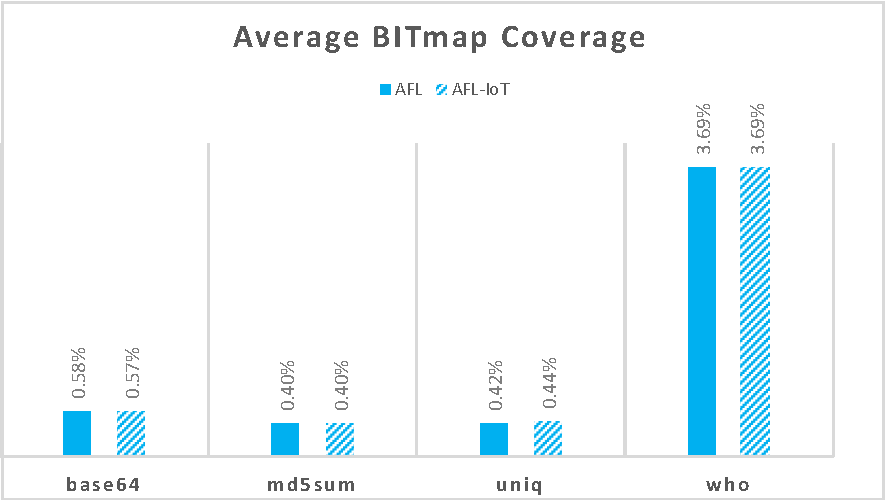
\includegraphics[width=\textwidth]{coverage}
%        \caption{Average Bitmap Coverage}
%    \end{subfigure}%
%\vspace{5pt}
\begin{subfigure}[b]{0.48\textwidth}
        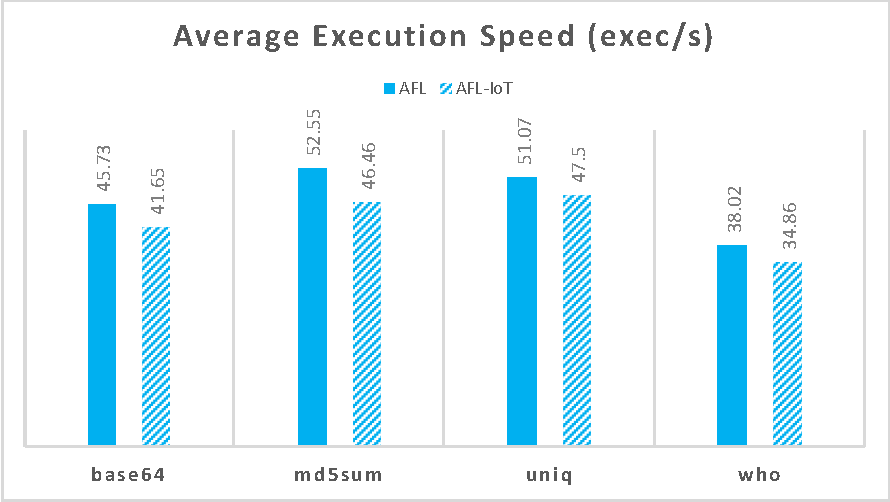
\includegraphics[width=\textwidth]{execspeed}
        \caption{Average Execution Speed}
    \end{subfigure}%

\caption{Performance Comparison Between AFL and \sysname.}
\label{figs:performance}
\end{figure}

\subsubsection{Performance}\label{sec:eval:performance}

In addition to correctness, performance is also vital for fuzzing. Since \sysname performs binary level instrumentation on target programs, it lacks source code level information, making instrumented code optimization even impossible. As a result, programs that instrumented at the binary level inevitably suffer from performance overhead in comparison with those with source code instrumentation. To evaluate \sysname, we compared the fuzzing test performance between source code level instrumentation by AFL and binary level instrumentation by \sysname. We again chose the LAVA-M dataset. This time we tested AFL and \sysname on all the four programs in LAVA-M with the same experiment environment as in our previous evaluation: dual-core CPU with 4GB memory under QEMU-ARM emulator. Similarly, for each target program, we built two versions: one compiled from source code with afl-clang and then run with AFL, another compiled with clang using the same parameters and then run with \sysname after binary level instrumentation. To mitigate the influence of randomness, we ran each version of the four program four times. The test of each running instance lasted for one hour on a single core.

We chose the number of total paths and execution speed as indicators of performance. Figure~\ref{figs:performance} compares the performance between AFL and \sysname. For all the four target programs, there is a 5\% average decrease for \sysname with instrumented programs in comparison with AFL with compiled programs in terms of number of total paths. The main reason of this decrease is that the instrumented programs ran slower than the compiled ones, resulting in a decrease in the number of instances that the fuzzer can execute in the same time. This affects the number of input that the fuzzer can mutate and therefore reduces the number of total paths.

%the version that instrumented by \sysname and the version AFL compiled from source code are almost consistent in terms of bitmap coverage.


%Recall that our instrumented version even gets a higher bitmap coverage In the $uniq$ test

%In the $uniq$ test, our instrumented version even gets a higher bitmap coverage. It should be noted that because \sysname uses the disassembler to locate basic blocks within the program, the result obtained is different from the what clang gets. Therefore, the ”bits” in the bitmap are not exactly the same of these two, it can only be a rough estimate of the coverage. 

Among all four programs in LAVA-M dataset, the instrumented versions have an execution speed drop of about 10\% on average compared with the compiled versions. This performance overhead can be attributed to the following three reasons:

\begin{enumerate}
    \item As \sysname performs instrumentation at binary level, it does not have enough context information, which makes it impossible to optimize the instrumented code stub. Therefore, \sysname must save all used registers every time when it enters the instrumented code stub. In contrast, AFL's source-based instrumentation can take full advantage of the compiler's optimization capabilities to avoid saving context frequently. Besides, it can also use idle registers to store data such as pointers globally, thus yielding a faster execution of instrumented code stubs.
    
    \item As mentioned in the design and implementation sections, we need to wrap the original instruction at the target address during the binary level instrumentation to ensure that the overwritten instruction can be executed as expected in the instrumented code segment. This inevitably introduces pivot-related operations together with expensive memory access instructions, which will slow down the execution of the target program.
    
    \item Finally, to guarantee the integrity of the original program, we place the instrumented code and data at the end of the entire program. 
    When loaded into the memory for execution, the program needs to jump to the instrumented code frequently to record the execution path. Since the original code segment of the program is far away from the instrumented code segment in memory, they cannot be loaded into the CPU cache at the same time. This frequent back and forth jump can cause a large number of instruction cache misses, which further adds additional overhead to the execution of the program.
\end{enumerate}

Overall, compared with AFL, \sysname achieves the similar code coverage performance, only about 5\% decrease in average number of total path and about 10\% decrease in average execution speed on binary programs. With slight performance overhead, \sysname is fully capable of fuzzing binary programs on most Linux-based IoT devices, where resources are very limited.

\subsection{Evaluation on Real-world IoT devices}\label{sec:eval:real}

The ultimate goal of \sysname is to fuzz binary programs in COTS Linux-based IoT devices. Since we have evaluated \sysname on benchmarks for its correctness and performance, next we can evaluate it on real-world IoT devices. Our evaluation selects 4 popular ARM Linux-based home routers from three well-known device manufacturer: ASUS AC1700, Xiaomi R1D/R3D and Netgear R7000. 


%Considering the popularity and the computational power, we pick three real-world COTS smart router, which are ASUS AC1700, Xiaomi R1D and Netgear R7000, as the target devices of our evaluation.

We upgraded all the four devices to the latest version of firmware and got shell access on each device using the debugging interfaces. Next, we selected dozens of command-line programs and daemon programs from each device. We determined how to interact with these programs and where to feed input to them by analyzing their behaviors. Since these programs are designed to run on these devices, they can be executed directly without further environment configuration or dependency resolution. For programs that read from the standard input or from a file, we performed binary level code instrumentation with with \sysname directly. For those designed to read input from network~(e.g. daemon programs), we additionally applied our approach described in Section~\ref{sec:design:daemons} to redirect the input to specific network interfaces and ports. Overall, our evaluation performed binary level instrumentation and fuzzing on over 100 binary programs on the four devices. For each fuzzing instance, we used a single-core CPU and ran within 24 hours.

\begin{table*}[htpb]
%\ttfamily
\scriptsize
\renewcommand\arraystretch{1.2}
\center
\begin{threeparttable}
\begin{tabular}
{
|C{0.05\textwidth}
|C{0.1\textwidth}
|C{0.1\textwidth}
|C{0.1\textwidth}
|C{0.06\textwidth}
|C{0.06\textwidth}
|C{0.06\textwidth}
|C{0.1\textwidth}
|C{0.1\textwidth}
|
}
%\toprule
\hline
\rmfamily\textbf{No.}&
\rmfamily\textbf{Binary Program}&
\rmfamily\textbf{Program Type}&
\rmfamily\textbf{Device}&
\rmfamily\textbf{Execution Time~(H)}&
\rmfamily\textbf{Branch Coverage}&
\rmfamily\textbf{Total Paths} &
\rmfamily\textbf{Execution Speed~(exec/s)} &
\rmfamily\textbf{Unique Crashes}
\\

\hline
1&	bunzip2\tnote{1}&   command-line&    Xiaomi R1D      &14&	2.27\%&	 203&	82  &	    11\\\hline
2&	bzcat\tnote{1}&	    command-line&    Xiaomi R1D      &12&	2.27\%&	 202&	111  &      13\\\hline
3&	gunzip\tnote{1}&	command-line&    ASUS AC1700             &14&	3.19\%&	 204&	35 &	    20\\\hline
4&	gzip\tnote{1}&	    command-line&    Netgear R7000            &12&	3.38\%&	 255&	124 &	    30\\\hline
5&	lzcat\tnote{1}&	    command-line&    Xiaomi R1D      &14&	0.96\%&	 78&	76&	        1\\\hline
6&	unlzma\tnote{1}&	command-line&    Xiaomi R1D      &12&	1.00\%&	 79&	94&	        4\\\hline
7&	zcat\tnote{1}&	    command-line&    Netgear R7000             &12&	3.23\%&	 224&	103&	    30\\\hline
8&	unzip&	            command-line&    ASUS AC1700              &12&	45.57\%&	 626&	278&	    12\\\hline
9&	tsar&	            command-line&    Xiaomi R1D      &14&	22.82\%&	 45&	22&	        14\\ \hline
10&	plugincenter&       network daemon & Xiaomi R1D  &14&	11.32\%&	262&	16&	        22\\\hline


\hline
\end{tabular}
\begin{tablenotes}
\footnotesize
\item[1] These programs are common Linux utilities that are integrated into a single executable called Busybox~\cite{busybox}. Since it combines many different programs in one executable, the branch coverage for each of them is relatively low.
\end{tablenotes}
\end{threeparttable}
\caption{\label{table:res_iot}Fuzzing Test Result in Real-world COTS Linux-based IoT Devices with \sysname.}
\end{table*}


Table~\ref{table:res_iot} shows the crashes that \sysname found in 10 different binary programs. The first seven programs are archive tools included in Busybox, a popular Linux utility toolbox for IoT devices. \sysname found as many as 30 unique crashes in these programs. Further analysis shows that most of the bugs have been fixed in the latest version of Busybox. Notably, one crash from lzcat and two crashes of unlzma were fixed just a few months before our evaluation, which demonstrates \sysname's ability to find real software bugs. In addition to the bugs in Busybox, \sysname also found 12 unique crashes in the independent archive program unzip. The ninth program in Table~\ref{table:res_iot} is a third-party version of sar~(System Activity Reporter)~\cite{sar}, in which \sysname found 14 unique crashes. The last one, plugincenter, is a daemon program from Xiaomi R1D smart router. Although daemon programs generally needs to do a series of initialization when starting, which could slow down the execution speed, \sysname still found 22 unique crashes in it.

In summary, \sysname is a fast, lightweight and easily deployable coverage-based fuzzing framework for binary programs on Linux-based IoT device. The major advantage of \sysname over other fuzzers is that it directly instruments the target program at the binary level, which makes it possible to fuzz various types of IoT devices with slight performance overhead. Our evaluation shows that \sysname is accurate and effective in finding bugs in binary programs on real world Linux-based IoT devices, and it only has about 10\% runtime overhead in comparison with AFL.